\subsubsection{Add a Diversity Term}
Providing several explanations that cover a range of diverse features rather than the ``the closest possible world'' maybe more helpful \cite{watcher2017}. For example, say that the quickest way to increase salary is changing the city, but Alice never thinks of moving to another city. Instead, she only wants to know what could happen if she further studies for a master degree. Diversity is required in the hope that the generation of several CFs for a single input data may increase the chance of an actionable CF to occur.

The choice of diversity metric should be careful because diversity could be reached by changes in numerous features or too fierce changes. Both situations are considered inappropriate \cite{DiCE}. Instead, the CFs should keep proximity with the input. \citeauthor{DiCE} \cite{DiCE} proposed to use the determinant of a kernel matrix as the diversity metric for n counterfactuals:
\begin{equation}\label{eq:dpp}
  dpp\_diversity(\mathbf{c_1,\dots,c_n})=\det(\mathbf{K}),\ \mathbf{K}_{i,j}=\frac{1}{1+dist(\mathbf{c_i,c_j})}
\end{equation}
%TODO: DPP的数学特征? OK
%This matrix is named after a widely adopted sampling method DPP (determinantal point processes). DPP focuses on sampling diverse contents and avoiding redundancy. In DPP context the matrix shown above is referred as a marginal kernel. Note that marginal kernel is a mathematical definition, and this specific form is not the only way to construct it. A key rule is, the more similar the chosen candidates are, the smaller the determinant of the kernel matrix will be. For detailed mathematical derivation the readers are redirected to the second chapter of \cite{kulesza2011dpp}.
%, here only an intuitional example is given.
\paragraph{dpp marginal kernel}
A DPP samples a subset \emph{A} of a discrete set \textbf{Y} with the following rule:
\begin{equation}\label{er:dpp}
  \mathcal{P}(A\subset\textbf{Y})=\det(K_A)
\end{equation}
which means the probability of choosing a certain subset equals to the minor of matrix \emph{K}, and \emph{K} is constructed by some relation of all elements in the complete set \textbf{Y}. Considering the simplest case with only two candidates \emph{i,j} in the subset, the possibility is:
\begin{equation}\label{eq:dpp1}
\begin{split}
  \mathcal{P}(i\in\textbf{Y})&=\det(K_{ii})=K_{ii}
\\
  \mathcal{P}(i,j\in\textbf{Y})&=\det\begin{pmatrix}
                                       K_{ii} & K_{ij} \\
                                       K_{ji} & K_{jj}
                                     \end{pmatrix}
                                      \\&=K_{ii}K_{jj}-K_{ij}K_{ji}
                                      \\&=\mathcal{P}(i\in\textbf{Y})\mathcal{P}(j\in\textbf{Y})-K_{ij}^2
\end{split}
\end{equation}
move a term to the left side we obtain the following equation, on the left side is exactly the definition of covariance:
\begin{equation}\label{eq:dpp2}
\begin{split}
  \mathcal{P}(i,j\in\textbf{Y})-\mathcal{P}(i\in\textbf{Y})\mathcal{P}(j\in\textbf{Y})=-K_{ij}^2
  \\\equiv Cov(i,j)=-K_{ij}^2
  \end{split}
\end{equation}
therefore, the possibility to choose a subset with two candidates equals the product of their independent possibility (marginal possibility) plus their (negative) covariance. The more relevant two candidates are, the higher $K_{ij}$ value is. When $\mathcal{P}(i),\mathcal{P}(j)$ are constants, a higher $K_{ij}$ value leads to a greater negative value of $\mathcal{P}(i,j)$ (i.e. the determinant of the matrix), which means a lower co-occurring chance. For 3-order matrix and higher, the explanation is no longer so intuitive. 
This term decreases when the CF candidates become more similar. For detailed mathematical derivation, the readers are redirected to \cite[second chapter]{kulesza2011dpp}.

Since multiple CFs are generated instead of only one, the basic formula needs to be modified before the diversity term is appended. The target loss and distance terms are averaged among all instances, a negative symbol is attached to diversity term because of the $\arg\min$ condition:
\begin{equation}\label{eq:DiCe}
\begin{split}
  \mathbf{C(x)}=\mathop{\arg\min}_{\mathbf{c_1,\dots,c_N}}&\frac{1}{N}\sum_{n=1}^{N}trgtloss(f(\mathbf{c_n}),y)
  +\frac{1}{N}\sum_{n=1}^{N}dist(\mathbf{c_n,x})
  \\&-dpp\_diversity(\mathbf{c_1,\dots,c_N})
\end{split}
\end{equation}

\subsubsection{Add a Data Distribution Term}
The CF generated by \autoref{eq:watcher} is not necessarily representative of the statistic data distribution \cite{FACE}. The first row of \autoref{fig:protoresult} is one example. Even though the generated CF obtained a different label number 3, it still looks like somehow in the between of number 3 and 5. Such poor explanation is less reliable, especially when in the vicinity of a decision boundary \cite{FACE}. Moreover, it may harm the user's interest. Consider the following example, Bob is told by the algorithm that he needs to replace his second-hand car with a new one if he wants to receive the loan. Bob knows that the solution is not \emph{plausible}, because for people with a poor credit history like him, buying a new car would not help. But he still purchased a new car on installment because it's advice from the bank. Later Bob's second loan application is denied again, and this time his credit score at the bank becomes even lower, because of the additional debt!

%One trivial solution, is abandoning data generation, instead choosing a closest case with the opposite label from a data bank \cite[conclusion]{bertossi2020asp}.
To handle with this issue, \citeauthor{prototype} \cite{prototype} propose a prototype loss term to measure the distance from the generated CF to other CF classes in latent layer. For each CF class \emph{i}, the algorithm firstly picks out the N nearest neighbours of the input that are classified as \emph{i}, then feeds them through an encoder and averages the output as the prototype of this CF class.
\begin{equation}\label{eq:prototype}
  proto_i=\frac{1}{N}\sum_{n=1}^{N}\mathbf{ENC}(\mathbf{x_n^i})
\end{equation}
Among all prototypes, the closest one to the input is chosen as the ``guidance'' for optimization:
\begin{equation}\label{eq:closestProto}
  j = {\arg\min}_{i\neq f(\textbf{x})}||\mathbf{ENC}(\textbf{x})-proto_i||_2
\end{equation}
The prototype loss term is defined as following:
\begin{equation}\label{eq:protoloss}
  prttyploss=||\mathbf{ENC}(\textbf{c})-proto_j||_2^2
\end{equation}
With the guidance of prototype, the perturbation is oriented to one chosen CF class rather than random search. The encoder used here could be any external known model, therefore requiring no internal information of the ``black-box'' model in question. We see that the closest target class to the input is chosen for a multiple classification task, this however could be revised for binary classification by explicitly choosing a target class. The generated CFs turn out to be more representative for their labels, as shown in \autoref{fig:protoresult}.

%\cite{prototype} furthermore shows that with the help of prototype loss term in searching, the target loss term could be dropped for improving efficiency. Generation methods based on loss function requires the gradient chain to know the optimization direction in next step. Unfortunately, as CF algorithms are often applied to "black-box" models, only the input data and the final prediction are available, the internal gradients are lost. Therefore, in order to measure the effect of a single perturbation of a feature \emph{k} on the final prediction, the gradient has to be approximated numerically by:
%\begin{equation}\label{eq:gradientNumerical}
%  \frac{\partial f_{pred}}{\partial x_k}\approx\frac{f_{pred}(x+\epsilon_k)-f_{pred}(x-\epsilon_k)}{2\epsilon}
%\end{equation}
%and this needs to be done on each feature in both directions for each gradient step, which results in numerous computation. For example, for a $28\times28$ MNIST image, the algorithm needs to call the model for $28\cdot28\cdot2$ times. Before, such numerous computation is still tolerated, because the target loss term ${trgtloss(f(\textbf{c}),y)}$ is the only roll that leads the generation to the target label. However, now the prototype loss term is also able to play the same guidance roll, and requires no internal information. The addition of ${prttyploss}$ significantly reduces both time and iterations about 80\%.

\begin{figure}
  \centering
  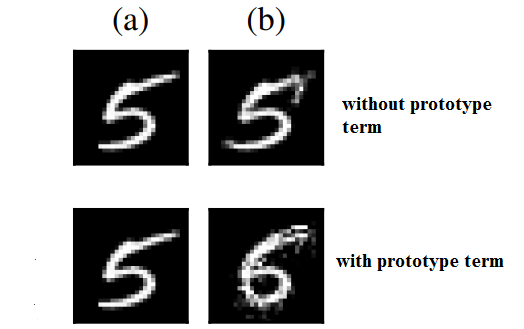
\includegraphics[width=0.5\textwidth]{proto.PNG}
  \caption{(a) column is the input data and (b) column is the CF output. In the first row, input class is 5 and CF class is 3. Second row, input class is 5 and CF class is 6. The addition of the prototype loss term generates a more interpretable CF. Credit: \cite{prototype}
  }
  \label{fig:protoresult}
\end{figure}

%The target loss term, in contrast, increases the time and results in a less interpretable CF, hence becomes a drawback in the whole formula and could be removed. 